\documentclass[11pt,a4paper]{ltjsarticle}
\usepackage{luatexja-fontspec}
\usepackage{geometry}
\usepackage{booktabs}
\usepackage{array}
\usepackage{enumitem}
\usepackage{graphicx}
\usepackage{amsmath}
\usepackage{fancyhdr}
\usepackage{xcolor}
\usepackage{hyperref}

\geometry{margin=24mm}
\setmainjfont[BoldFont=Hiragino Kaku Gothic ProN]{Hiragino Mincho ProN}
\setsansjfont{Hiragino Kaku Gothic ProN}
\setmonofont{Menlo}
\hypersetup{colorlinks=true, linkcolor=blue!55!black, urlcolor=blue!55!black}

\pagestyle{fancy}
\fancyhf{}
\lhead{研究進捗報告}
\rhead{2026 年 7 月 14 日}
\cfoot{\thepage}
\renewcommand{\headrulewidth}{0.2pt}

\newcommand{\rk}{\textrm{Recall@}K}
\setlist{nosep}

\begin{document}

\begin{center}
{\sffamily\large 物理モデルの自動構築：設計した特徴量はなぜ効くのか\\——精度向上の分解と、効く場所の特定}
\end{center}
\vspace{0.3em}
\hfill 作成者：M2\ 一洋
\vspace{0.8em}

%======================================================================
\section{前回ゼミレビュー}
%======================================================================
\textbf{研究の目的}：科学文献から数式を集めておき、「どんな物理モデルを作りたいか」（説明文と入出力変数）を入力すると、そのモデルを構成するのに必要な\textbf{数式の集合}を提示する。


  前回は、データベースを 11,146 式・2,838 ケースに拡大し、層化分割・DAE ケースの再生成を行なった。その上で、文章類似度など基本 7 特徴量に\textbf{集合特徴量} 3 個を加えた計 10 特徴量を多層パーセプトロン（MLP）で学習し、候補の式を並べ直す本手法（reranker-10S）を構築した。$\rk$（物理モデルの正解式数 $K$ に合わせ、上位 $K$ 件に入った正解の割合）を設定 A（オリジナル＋文献横断＋DAE、1{,}823 件）で $0.521\to0.743$（$+0.222$）、設定 B（DAE のみ 1{,}000 件）で $0.466\to0.689$ に改善し、全設定で本手法＞baseline（古典的情報検索手法）＞ LLM 直接生成となることを報告した。
  


%======================================================================
\section{今回の進捗}
%======================================================================
これに対し\textbf{加藤先生から「設計した特徴量はなぜ、学習精度向上に効くのかの考察が重要」とのご指摘}をいただいた。本報告では、この「なぜ」を実験で調べた。

（古典的検索手法と比べた）精度向上 $+0.222$ は、次の 3 段に分解できた。baseline は\textbf{文章類似度と変数の一致度の 2 特徴量を、固定の重み（7:3）で足すだけ}の方式である。(a) 同じ 2 特徴量のまま\textbf{重み付けを固定から MLP の学習に変える}と $0.521\to0.601$（$+0.080$）。(b) \textbf{特徴量を 2 個から 7 個に増やす}と $0.601\to0.693$（$+0.092$）。(c) \textbf{集合特徴量 3 個を加える}と $0.693\to0.743$（$+0.050$）。さらに特徴量を 1 つずつ調べると、精度を上げるのは\textbf{変数の重なりを見る特徴量}だけで、\textbf{話題の近さを見る特徴量（意味の近さ・分野の一致）はどの形でも効かない}ことが分かった。集合特徴量の効果は複数式・多変数のケースで大きい（\S\ref{sec:exp1}）。
  

%======================================================================
\section{実験：どの特徴量が・どんなケースで効くのか}\label{sec:exp1}
%======================================================================
\textbf{方法}：どの特徴量が効くかを見るため、\textbf{特徴量を 1 つだけ土台に足したときの $\rk$ の変化}を測った。土台は 2 つ用意した。土台 A は baseline と同じ 2 特徴量（文章類似度・変数の一致度）を MLP で学習したもの、土台 B は基本 7 特徴量を学習したものである。土台 A には残る 5 個の基本特徴量を、土台 B には集合特徴量 3 個を、それぞれ 1 つずつ足した。各特徴量の定義は表~\ref{tab:features} に示す。集合特徴量の効果を正解式数・入力変数数で層別した（図~\ref{fig:fingerprint}）。

\begin{table}[h]\centering
\small
\caption{10 個の特徴量の定義。式の変数を $V_e$、クエリ（入力）の入出力変数を $V_q$（入力 $V_{\mathrm{in}}$・出力 $V_{\mathrm{out}}$）、既に選んだ式集合の変数を $V_S$ とする。}
\label{tab:features}
\begin{tabular}{@{}lp{0.66\linewidth}@{}}
\toprule
特徴量 & 定義 \\
\midrule
\multicolumn{2}{@{}l}{\textbf{基本特徴量（7 個）：各式を単独で評価}}\\
文章類似度 & 説明文と式まわりの文章の単語の重なり（TF-IDF のコサイン類似度） \\
変数の一致度 & 入出力変数と式の変数の重なり $|V_q\cap V_e|/|V_q\cup V_e|$（Jaccard 係数） \\
意味の近さ & 説明文と式を意味空間（SVD）に埋め込んだときのコサイン類似度 \\
入力変数の被覆 & 入力変数のうち式に現れる割合 $|V_{\mathrm{in}}\cap V_e|/|V_{\mathrm{in}}|$ \\
出力変数の被覆 & 出力変数のうち式に現れる割合 $|V_{\mathrm{out}}\cap V_e|/|V_{\mathrm{out}}|$ \\
式の特化度 & 式の変数のうち入出力変数が占める割合 $|V_q\cap V_e|/|V_e|$（無関係な変数を持たない式ほど高い） \\
分野の一致 & 式の分野が説明文に現れれば 1、なければ 0 \\
\addlinespace
\multicolumn{2}{@{}l}{\textbf{集合特徴量（3 個）：既に選んだ式集合（第 1 段で上位に来た数件）を基準に評価}}\\
補完性 & まだ覆えていない入出力変数を新たに補う割合 $|(V_q\cap V_e)\setminus V_S|/|V_q|$ \\
一貫性 & 式の変数のうち既選択集合と共有する割合 $|V_e\cap V_S|/|V_e|$ \\
分野の一致（集合版） & 既選択集合のうち候補と同じ分野の式の割合 \\
\bottomrule
\end{tabular}
\end{table}

\begin{table}[h]\centering
\small
\caption{特徴量を 1 つだけ土台に足したときの $\rk$（1{,}823 ケース・乱数 10 通り）。差は直上の土台からの差、$p$ は乱数を対応させた $t$ 検定。}
\label{tab:ablation}
\begin{tabular}{lccc}
\toprule
方式・追加した特徴量 & $\rk$ & 土台からの差 & $p$ 値 \\
\midrule
baseline（2 特徴量・固定重み・学習なし） & $0.521$ & — & — \\
\midrule
\textbf{土台 A：2 特徴量を MLP で学習} & $0.601$ & — & — \\
\quad ＋意味の近さ（SVD） & $0.599$ & $-0.002$ & $0.48$ \\
\quad ＋入力変数の被覆 & $0.620$ & $+0.019$ & $<0.001$ \\
\quad ＋出力変数の被覆 & $0.607$ & $+0.006$ & $0.002$ \\
\quad ＋式の特化度 & $\mathbf{0.691}$ & $\mathbf{+0.090}$ & $<0.001$ \\
\quad ＋分野の一致 & $0.603$ & $+0.002$ & $0.06$ \\
\midrule
\textbf{土台 B：基本 7 特徴量を MLP で学習} & $0.693$ & — & — \\
\quad ＋補完性 & $0.745$ & $+0.052$ & $<0.001$ \\
\quad ＋一貫性 & $0.743$ & $+0.050$ & $<0.001$ \\
\quad ＋分野の一致（集合版） & $0.693$ & $-0.000$ & $0.98$ \\
\midrule
本手法 reranker-10S（7 ＋ 集合 3 特徴量） & $0.743$ & — & — \\
\bottomrule
\end{tabular}
\end{table}

\textbf{結果}（表~\ref{tab:ablation}・図~\ref{fig:fingerprint}）：
\begin{itemize}[leftmargin=1.5em]
  \item \textbf{基本特徴量の内訳（土台 A から）}：$+0.092$ のほぼ全部を\textbf{式の特化度 1 個}が担う（$0.601\to0.691$、$+0.090$）。この 1 個だけで 7 特徴量すべて（$0.693$）にほぼ届く。入力変数の被覆（$+0.019$）・出力変数の被覆（$+0.006$）は小さく、\textbf{意味の近さ（SVD）は効果がない}（$-0.002$、$p=0.48$）。
  \item \textbf{話題の近さはどの形でも効かない}：分野の一致は、基本特徴量として足しても（$+0.002$、$p=0.06$）、集合特徴量として足しても（$-0.000$、$p=0.98$）変わらない。意味の近さ（SVD）も効かない（$p=0.48$）。効くのはいずれも変数の重なりを測る特徴量であった。
  \item \textbf{集合特徴量は組合せが難しいときに効く（土台 B から）}：補完性・一貫性を足す効果は、正解式数 1 のケースでは 0、2〜3 式で最大（$+0.07$〜$+0.12$）。入力変数数では 6 個以下で 0、7〜15 個で最大（$+0.07$〜$+0.09$）、\textbf{16 個以上では $+0.035$ に縮む}（図~\ref{fig:fingerprint}）。
  \item \textbf{独立の手法（順列特徴量重要度）でも同じ結論（図~\ref{fig:pfi}）}：土台を複数作るのでなく、最良モデル 1 つで各特徴量を壊した（値をシャッフルした）ときの $\rk$ の低下を測ると、\textbf{変数の重なりを測る 6 特徴量をまとめて壊すと $0.743\to0.065$ に崩れ}（$-0.678$、$p<0.001$）、\textbf{話題を測る 4 特徴量をまとめて壊してもほとんど変わらない}（$-0.006$、有意でない）。原理の異なる 2 手法（再訓練するアブレーションと、壊すだけの順列重要度）が同じ結論に至る。
\end{itemize}


\begin{figure}[h]\centering
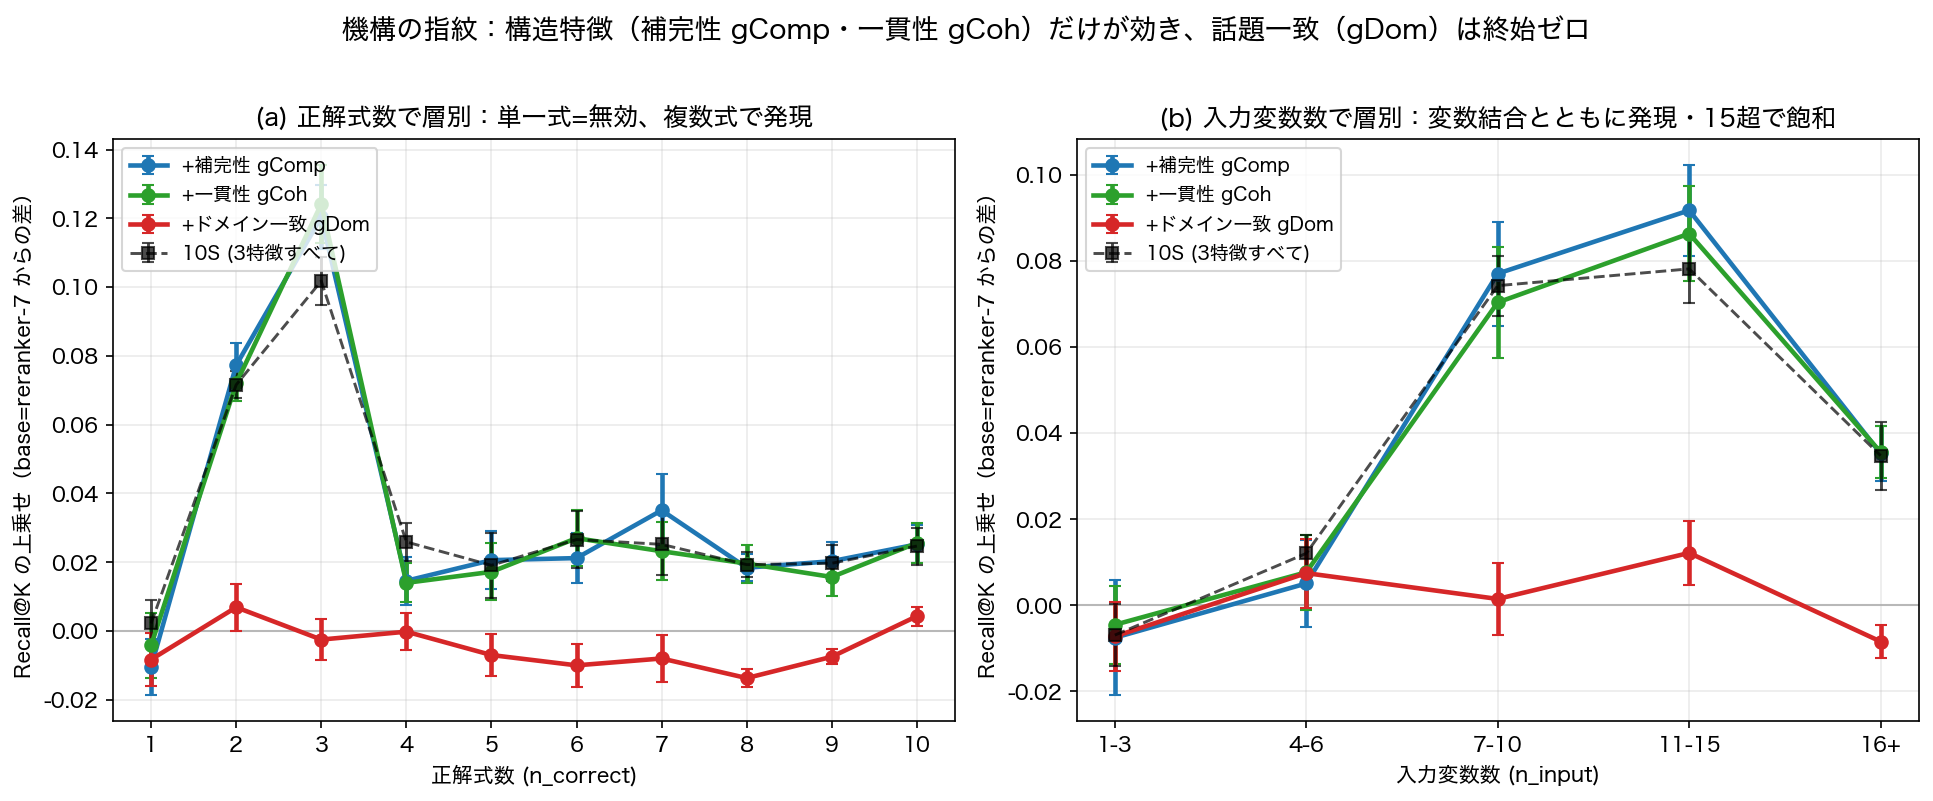
\includegraphics[width=\linewidth]{figures/fig_mechanism_fingerprint.png}
\caption{集合特徴量を土台 B（基本 7 特徴量）に 1 つ足したときの $\rk$ の変化。(a) 正解式数別、(b) 入力変数数別。補完性（青）・一貫性（緑）は複数式・多変数の層でのみ正の効果を持ち、分野の一致〔集合版〕（赤）は全層で 0 付近である。}
\label{fig:fingerprint}
\end{figure}

\begin{figure}[h]\centering
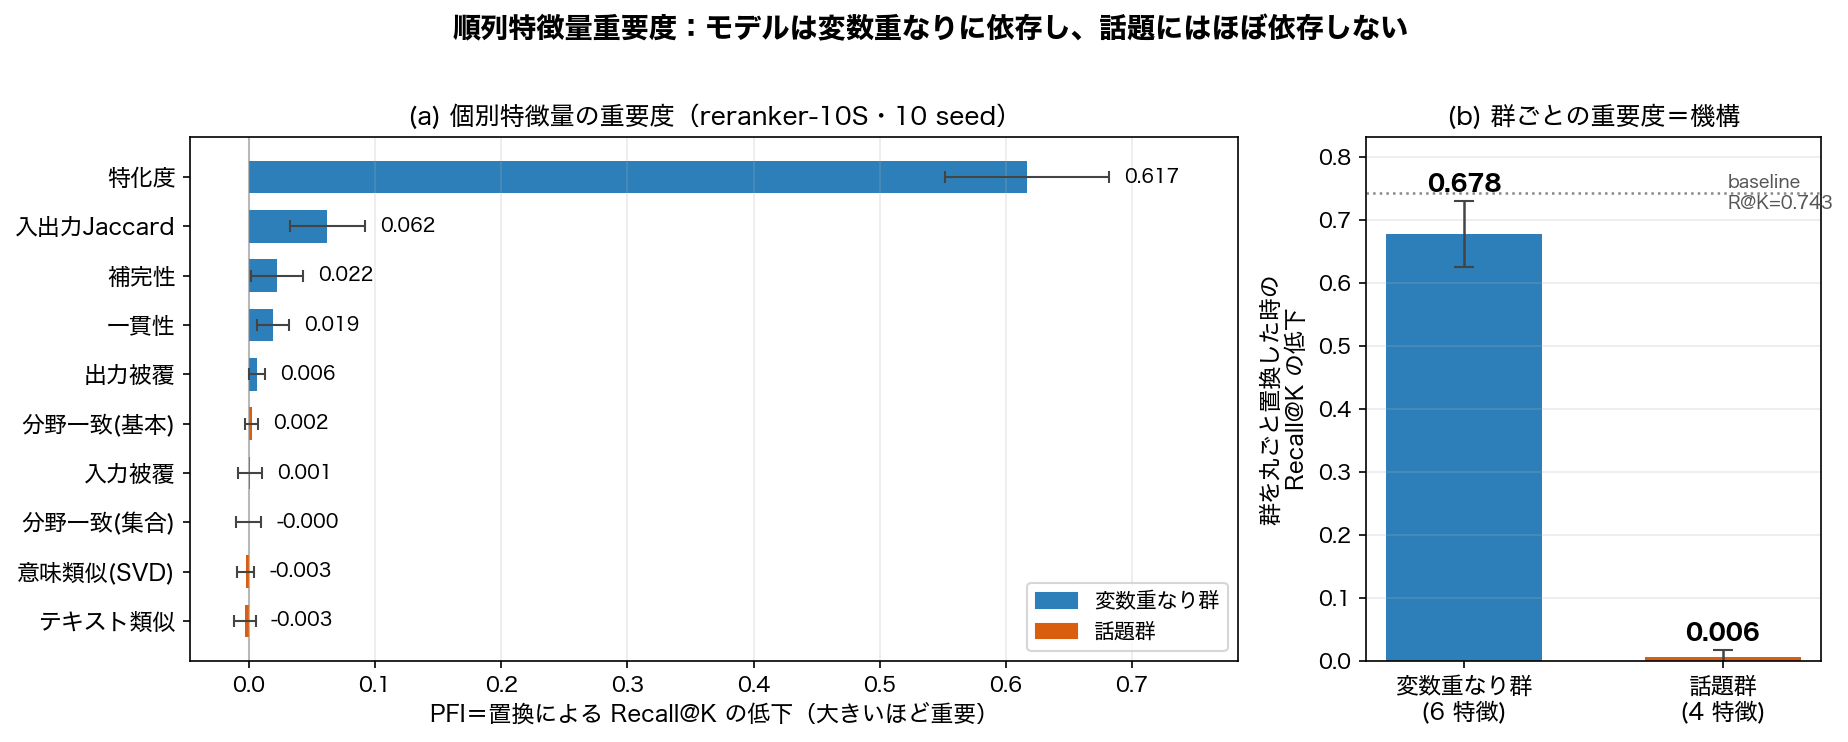
\includegraphics[width=\linewidth]{figures/fig_pfi_importance.png}
\caption{最良モデル reranker-10S の順列特徴量重要度（10 seed の平均 $\pm$ 標準偏差。重要度＝その特徴量の値をケース内でシャッフルしたときの $\rk$ の低下）。(a) 特徴量ごと（色は群）、(b) 変数の重なり群 vs 話題群を丸ごと壊した場合（点線は元の $\rk=0.743$）。モデルは変数の重なりに依存し、話題はほとんど使っていない。}
\label{fig:pfi}
\end{figure}

%======================================================================
\section{考察：何が分かったか}\label{sec:discussion}
%======================================================================
\begin{enumerate}[leftmargin=1.8em]
  \item \textbf{本課題は「説明文に似た式を探す」検索ではない}：効いた特徴量がすべて変数の重なりを測るもので、文章・話題の近さ（意味の近さ・分野の一致）はどの形でも効かなかった。つまり、古典的検索や LLM 直接生成が頼る文章・話題の類似では本課題は解けず、\textbf{「同じ変数を持つ式」を選ぶこと}が要る（前回、両者とも本手法に劣った）。
  \item \textbf{さらに、式は集合として組み立てる必要がある}：式どうしの組合せを見る集合特徴量が複数式・多変数のケースで効くこと（図~\ref{fig:fingerprint}）、および LLM 直接生成が必要な式を作れても上位 $K$ 件に組めないこと（前回報告）は、物理モデルの構築が式を 1 本ずつ選ぶだけでなく\textbf{変数を補い合う集合として組み立てる}側面を持つことを示す。
  \item \textbf{限界}：(i) 特徴量の追加 $+0.092$ はほぼ式の特化度 1 個に由来し、集合特徴量の効果（$+0.050$）はそれより小さい。(ii) 16 変数以上で集合特徴量の効果が縮む原因（補完性の基準の固定）は推定である。
\end{enumerate}

%======================================================================
\section{まとめと今後の課題}
%======================================================================
\textbf{今回}：前回の改善 $+0.222$ を 3 段（重み付けの学習 $+0.080$・特徴量の追加 $+0.092$・集合特徴量 $+0.050$）に分解し、全特徴量を 1 つずつ評価して、\textbf{精度を上げるのは変数の重なりを測る特徴量に限られる}ことを示した。

\textbf{今後の課題}：
\begin{itemize}[leftmargin=1.5em]
  \item 修士論文の骨子（作成済み）を加藤先生と相談しながら修正。
  \item 論文のロジックを補完するための追加実験を行う。
\end{itemize}

\end{document}
